\documentclass[11pt]{article}
\textwidth 15.9cm
\textheight 23. cm
\addtolength{\oddsidemargin}{-11.5mm}
\addtolength{\evensidemargin}{-11.5mm}
\addtolength{\topmargin}{-19.0mm}

%\usepackage{amsmath}
\usepackage[ansinew]{inputenc}
\usepackage[bbgreekl]{mathbbol}
\usepackage{amsmath,amssymb}
\usepackage{graphicx}
\usepackage{hyperref}
\usepackage{url}
\usepackage[numbers,square]{natbib}
\usepackage{multirow}
\usepackage{bbm}
\usepackage{authblk}
\usepackage{subcaption}
\renewcommand{\Affilfont}{\footnotesize}
%\renewcommand{\Authfont}{\normalsize}

%\usepackage{stmaryrd}
\usepackage{comment}
\usepackage{showlabels}
\usepackage{soul}

%%%%%%%% MACROS
\include{GempicLatexMacros}

\newcommand{\hi}{\hat{i}}
\newcommand{\hj}{\hat{j}}
\newcommand{\hk}{\hat{k}}

% \newcommand{\arr}[1]{{\bs{\mathsf{#1}}}}

\newtheorem{theorem}{Theorem}
\newtheorem{lemma}{Lemma}
\newtheorem{remark}{Remark}
\newtheorem{definition}{Definition}
\newtheorem{assumption}{Assumption}

\begin{document}

\section{Multi-Dimensional de Rham Complexes}

\subsection{The 3D de Rham Complex}

As explained in Section \ref{sec:Maxwell_with_discrete_forms}
the fields in GEMPIC are based on the 3D de Rham sequence

\begin{figure}[h]
\centering
	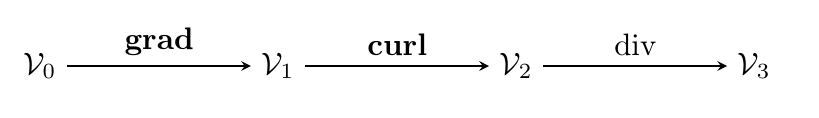
\includegraphics[width=.6\textwidth]{deRham3D.png}
\end{figure}
where $$\mathcal{V}_0 \subset H^1(\Omega),\ \mathcal{V}_1 \subset H(\textbf{curl};\Omega),\ \mathcal{V}_2 \subset H(\text{div};\Omega), \ \mathcal{V}_3 \subset L^2(\Omega)$$ are conforming subspaces. Each element of these spaces is uniquely determined by the degrees of freedom (DOFs), i.e. nodal values for $\mathcal{V}_0$, edge integrals for $\mathcal{V}_1$, face integrals for $\mathcal{V}_2$, and cell integrals for $\mathcal{V}_3$. In addition, a field can either belong to the primal or the dual complex.

In the code, fields are initialized by a command of the form
\begin{center} \verb|DeRhamField<Grid, Space>|\end{center}
where 
\begin{itemize}
	\item \verb|Grid| is either \verb|primal| or \verb|dual|
	\item \verb|Space| is either \verb|node|, \verb|edge|, \verb|face|, or \verb|cell|
\end{itemize}
in accordance to the DOFs.

\subsection{The Stacked de Rham Complex in 2D}
\label{sec:stacked_deRham2D}

In 2D (all fields only depend on $x$ and $y$) there are two de Rham sequences:

\begin{figure}[h]
\centering
	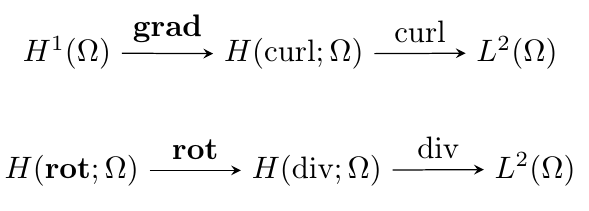
\includegraphics[width=.3\textwidth]{deRham2D.png}
\end{figure}
where the 2D operators curl and $\mathbf{rot}$ are defined by
$$
\text{curl} \begin{pmatrix} E_x \\ E_y \end{pmatrix} = \partial_x E_y - \partial_y E_x,
$$ 
$$
\mathbf{rot} (E_z) = \begin{pmatrix} \partial_y E_z \\ -\partial_x E_z \end{pmatrix}.
$$
In the code, these two sequences are embedded into the 3D complex by stacking them in the following way:
\begin{figure}[h]
\centering
	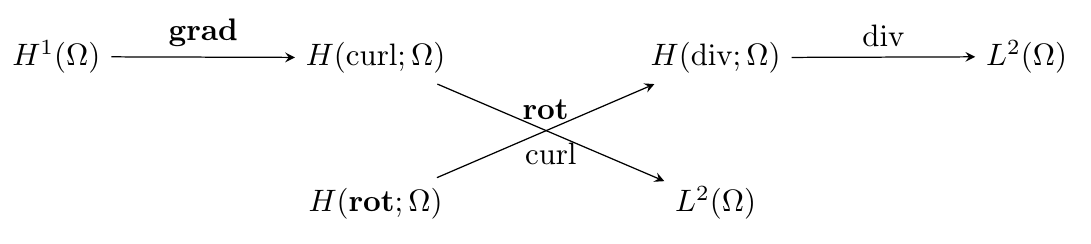
\includegraphics[width=.7\textwidth]{deRham2Dstacked.png}
\end{figure}
This means that in each $\mathcal{V}_i$ the fields have the same number of components as in 3D, the spaces are given by
$$\mathcal{V}_0 = H^1(\Omega), \hspace{.5cm} \mathcal{V}_1 = \begin{pmatrix} H(\text{curl};\Omega)\\ H(\textbf{rot};\Omega) \end{pmatrix}, \hspace{.5cm} \mathcal{V}_2 = \begin{pmatrix} H(\text{div};\Omega)\\ L^2(\Omega) \end{pmatrix}, \hspace{.5cm} \mathcal{V}_3 = L^2(\Omega),$$
and the differential operators are
\begin{align*}
	\text{grad} (\varphi) &= \begin{pmatrix} \partial_x \varphi \\ \partial_y \varphi \\ 0 \end{pmatrix},\\
	\textbf{curl} \begin{pmatrix} E_x \\ E_y \\ E_z \end{pmatrix} &= \begin{pmatrix} \mathbf{rot}(E_z) \\ \text{curl} \begin{pmatrix} E_x \\ E_y \end{pmatrix} \end{pmatrix},\\
	\text{div} \begin{pmatrix} B_x \\ B_y \\ B_z \end{pmatrix} &= \partial_x B_x + \partial_y B_y.
\end{align*}
This way, any code written for 3D works without any modifications to the fields just the same in 2D. A \verb|DeRhamField| defined on \verb|Space::edge| is still in $\mathcal{V}_1$, the only difference is that the third component will be node centered, since it belongs to $H(\mathbf{rot}; \Omega)$.

\subsection{The Stacked de Rham Complex in 1D}
\label{sec:stacked_deRham1D}

In 1D (all fields only depend on $x$) the implementation follows the same lines. There is only one de Rham sequence

\begin{figure}[h]
\centering
	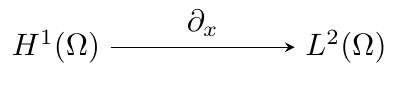
\includegraphics[width=.3\textwidth]{deRham1D.png}
\end{figure}
which is embedded into 3D complex in the following way:
\begin{figure}[h]
\centering
	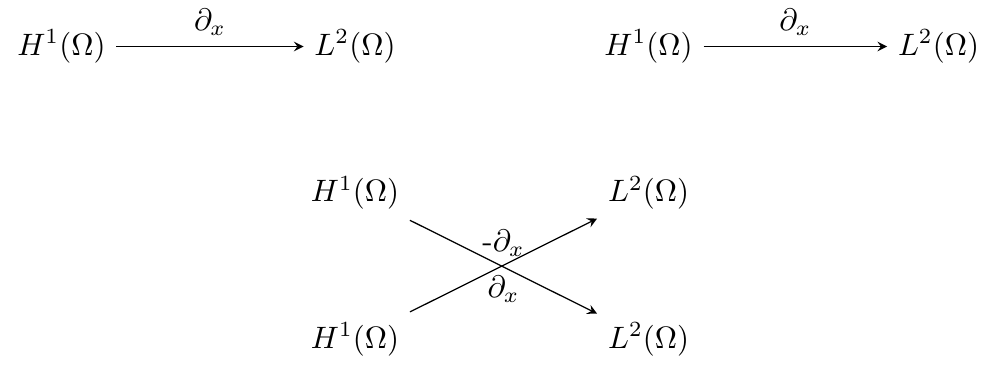
\includegraphics[width=.7\textwidth]{deRham1Dstacked.png}
\end{figure}

Again, the fields have the same number of components as in 3D, the spaces are now given by
$$\mathcal{V}_0 = H^1(\Omega), \hspace{.5cm} \mathcal{V}_1 = \begin{pmatrix} L^2(\Omega)\\ H^1(\Omega) \\H^1(\Omega) \end{pmatrix}, \hspace{.5cm} \mathcal{V}_2 = \begin{pmatrix} H^1(\Omega)\\ L^2(\Omega) \\ L^2(\Omega) \end{pmatrix}, \hspace{.5cm} \mathcal{V}_3 = L^2(\Omega)$$
and the differential operators are
\begin{align*}
	\text{grad} (\varphi) &= \begin{pmatrix} \partial_x \varphi \\ 0 \\ 0 \end{pmatrix},\\
	\textbf{curl} \begin{pmatrix} E_x \\ E_y \\ E_z \end{pmatrix} &= \begin{pmatrix} 0 \\ -\partial_x E_z \\ \partial_x E_y \end{pmatrix},\\
	\text{div} \begin{pmatrix} B_x \\ B_y \\ B_z \end{pmatrix} &= \partial_x B_x.
\end{align*}
This way, any code written for 3D works without any modifications to the fields just the same in 1D. A \verb|DeRhamField| defined on \verb|Space::edge| is still in $\mathcal{V}_1$, the only difference is that the second and third component will be node centered, since they belong to $H^1(\Omega)$.


\subsection{Degrees of Freedom in 3D}

The degrees of freedom in 3D were defined in Section \ref{sec:dofs_and_reductions}.

\subsection{Degrees of Freedom in 2D}
\label{sec:dofs_2D}

In 2D, we assume that all the functions are constant along $z$.


\subsubsection{2D Primal Degrees of Freedom}

According to the above stacked de Rham sequence, we define

\begin{itemize}
    \item $\mathcal{R}^{2D}_0(\phi)_{i,j} := \phi(x_i,y_j)$
\end{itemize}
for the degrees of freedom in $\mathcal{C}_0^{2D}$,
\begin{itemize}
    \item $\mathcal{R}^{2D,x}_1(E_x)_{\iph,j} := \int_{x_i}^{x_{i+1}} E_x(x,y_j)\dd x $
    \item $\mathcal{R}^{2D,y}_1(E_y)_{i,\jph} := \int_{y_j}^{y_{j+1}} E_y(x_i,y)\dd y $
    \item $\mathcal{R}^{2D,z}_1(E_z)_{i,j} := E_z(x_i,y_j)$
\end{itemize}
for the degrees of freedom in $\mathcal{C}_1^{2D}$,
\begin{itemize}
    \item $\mathcal{R}^{2D,x}_2(B_x)_{i,\jph} := \int_{y_j}^{y_{j+1}} B_x(x_i,y)\dd y $
    \item $\mathcal{R}^{2D,y}_2(B_y)_{\iph,j} := \int_{x_i}^{x_{i+1}} B_y(x,y_j)\dd x $
    \item $\mathcal{R}^{2D,z}_2(B_z)_{\iph,\jph} := \int_{x_i}^{x_{i+1}}\int_{y_j}^{y_{j+1}} B_z(x,y)\dd x\dd y $
\end{itemize}
for the degrees of freedom in $\mathcal{C}_2^{2D}$,
and 
\begin{itemize}
    \item $\mathcal{R}^{2D}_3(f)_{\iph,\jph} := \int_{x_i}^{x_{i+1}}\int_{y_j}^{y_{j+1}} f(x,y)\dd x\dd y $
\end{itemize}
for the degrees of freedom in $\mathcal{C}_3^{2D}$,

\subsubsection{2D Dual Degrees of Freedom}

We define
\begin{itemize}
    \item $\tilde{\mathcal{R}}^{2D}_0(g)_{\iph,\jph} := g(x_\iph,y_\jph)$
\end{itemize}
for the degrees of freedom in $\tilde{\mathcal{C}}_0^{2D}$,
\begin{itemize}
    \item $\tilde{\mathcal{R}}^{2D,x}_1(H_x)_{i,\jph} := \int_{x_\imh}^{x_{\iph}} H_x(x,y_\jph)\dd x $
    \item $\tilde{\mathcal{R}}^{2D,y}_1(H_y)_{\iph,j} := \int_{y_\jmh}^{y_{\jph}} H_y(x_\iph,y)\dd y $
    \item $\tilde{\mathcal{R}}^{2D,z}_1(H_z)_{\iph,\jph} := H_z(x_\iph,y_\jph) $
\end{itemize}
for the degrees of freedom in $\tilde{\mathcal{C}}_1^{2D}$,
\begin{itemize}
    \item $\tilde{\mathcal{R}}^{2D,x}_2(D_x)_{\iph,j} := \int_{y_\jmh}^{y_{\jph}} D_x(x_\iph,y)\dd y  $
    \item $\tilde{\mathcal{R}}^{2D,y}_2(D_y)_{i,\jph} := \int_{x_\imh}^{x_{\iph}} D_y(x,y_\jph)\dd x  $
    \item $\tilde{\mathcal{R}}^{2D,z}_2(D_z)_{i,j} := \int_{x_\imh}^{x_{\iph}} \int_{y_\jmh}^{y_{\jph}} D_z(x,y)\dd x \dd y $
\end{itemize}
for the degrees of freedom in $\tilde{\mathcal{C}}_2^{2D}$,
and
\begin{itemize}
	\item $\tilde{\mathcal{R}}^{2D}_3(\rho)_{i,j} := \int_{x_\imh}^{x_{\iph}} \int_{y_\jmh}^{y_{\jph}} \rho(x,y)\dd x \dd y$
\end{itemize}
for the degrees of freedom in $\tilde{\mathcal{C}}_3^{2D}$.

\subsection{Degrees of Freedom in 1D}
\label{sec:dofs_1D}

In 1D, we assume that all the functions are constant along $y$ and $z$.

\subsubsection{1D Primal Degrees of Freedom}

According to the above stacked de Rham sequence, we define
\begin{itemize}
    \item $\mathcal{R}^{1D}_0(\phi)_{i} := \phi(x_i)$
\end{itemize}
for the degrees of freedom in $\mathcal{C}_0^{1D}$,
\begin{itemize}
    \item $\mathcal{R}^{1D,x}_1(E_x)_{\iph} := \int_{x_i}^{x_{i+1}} E_x(x)\dd x $
    \item $\mathcal{R}^{1D,y}_1(E_y)_{i} := E_y(x_i) $
    \item $\mathcal{R}^{1D,z}_1(E_z)_{i} := E_z(x_i)$
\end{itemize}
for the degrees of freedom in $\mathcal{C}_1^{1D}$,
\begin{itemize}
    \item $\mathcal{R}^{1D,x}_2(B_x)_{i} := B_x(x_i)$
    \item $\mathcal{R}^{1D,y}_2(B_y)_{\iph} := \int_{x_i}^{x_{i+1}} B_y(x)\dd x $
    \item $\mathcal{R}^{1D,z}_2(B_z)_{\iph} := \int_{x_i}^{x_{i+1}} B_z(x)\dd x $
\end{itemize}
for the degrees of freedom in $\mathcal{C}_2^{1D}$,
and 
\begin{itemize}
    \item $\mathcal{R}^{1D}_3(f)_{\iph} := \int_{x_i}^{x_{i+1}} f(x)\dd x $
\end{itemize}
for the degrees of freedom in $\mathcal{C}_3^{1D}$.

\subsubsection{1D Dual Degrees of Freedom}

We define
\begin{itemize}
    \item $\tilde{\mathcal{R}}^{1D}_0(g)_{\iph} := g(x_\iph)$
\end{itemize}
for the degrees of freedom in $\tilde{\mathcal{C}}_0^{1D}$,
\begin{itemize}
    \item $\tilde{\mathcal{R}}^{1D,x}_1(H_x)_{i} := \int_{x_\imh}^{x_{\iph}} H_x(x)\dd x $
    \item $\tilde{\mathcal{R}}^{1D,y}_1(H_y)_{\iph} := H_y(x_\iph)$
    \item $\tilde{\mathcal{R}}^{1D,z}_1(H_z)_{\iph} := H_z(x_\iph) $
\end{itemize}
for the degrees of freedom in $\tilde{\mathcal{C}}_1^{1D}$,
\begin{itemize}
    \item $\tilde{\mathcal{R}}^{1D,x}_2(D_x)_{\iph} := D_x(x_\iph) $
    \item $\tilde{\mathcal{R}}^{1D,y}_2(D_y)_{i} := \int_{x_\imh}^{x_{\iph}} D_y(x)\dd x  $
    \item $\tilde{\mathcal{R}}^{1D,z}_2(D_z)_{i} := \int_{x_\imh}^{x_{\iph}} D_z(x)\dd x  $
\end{itemize}
for the degrees of freedom in $\tilde{\mathcal{C}}_2^{1D}$,
and
\begin{itemize}
	\item $\tilde{\mathcal{R}}^{1D}_3(\rho)_{i} := \int_{x_\imh}^{x_{\iph}} \rho(x)\dd x $
\end{itemize}
for the degrees of freedom in $\tilde{\mathcal{C}}_3^{1D}$.


\end{document}